\begin{enumerate}[label={Aufgabe H\arabic*},start=20]
	\item 
		\begin{enumerate}
			\item \textbf{SRPT} \blanko

				\begin{center}
					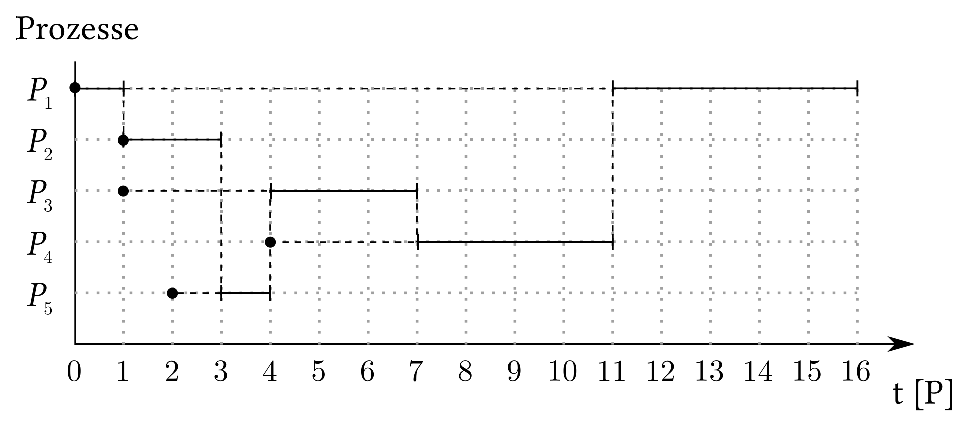
\includegraphics[width=0.7\textwidth]{20a.eps}
				\end{center}
			\item \textbf{RR} \blanko

				\begin{center}
					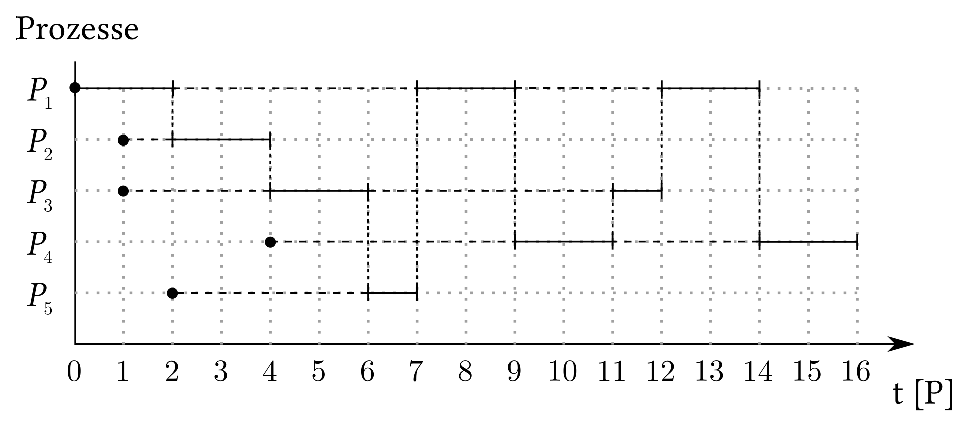
\includegraphics[width=0.7\textwidth]{20b.eps}
				\end{center}

			\item \textbf{SRPT}
				\vspace{1em}
				\begin{center}
					\renewcommand*{\arraystretch}{1.2}
					\begin{tabular}{@{}lllllll@{}}
						\toprule
						{\small Proz.} & {\small Ankunftz.} & {\small Bedienz.} & {\small Beendigungsz.} & {\small Verweildauer} & {\small Wartezeit} \\
						\midrule
						$P_1$ & $0$ & $6$ & $16$ & $16$ & $10$ \\
						$P_2$ & $1$ & $2$ & $3$ & $2$ & $0$ \\
						$P_3$ & $1$ & $3$ & $7$ & $6$ & $3$ \\
						$P_4$ & $4$ & $4$ & $11$ & $7$ & $3$ \\
						$P_5$ & $2$ & $1$ & $4$ & $2$ & $1$ \\
						\bottomrule
					\end{tabular}
				\end{center}
				\vspace{1em}

				Mittlere Verweildauer $ = (16+2+6+7+2)/5 = 6,60$ \\
				Mittlere Wartezeit $ = (10+0+3+3+1)/5 = 3.40$

				\textbf{RR}
				\vspace{1em}
				\begin{center}
					\renewcommand*{\arraystretch}{1.2}
					\begin{tabular}{@{}lllllll@{}}
						\toprule
						{\small Proz.} & {\small Ankunftz.} & {\small Bedienz.} & {\small Beendigungsz.} & {\small Verweildauer} & {\small Wartezeit} \\
						\midrule
						$P_1$ & $0$ & $6$ & $14$ & $14$ & $8$ \\
						$P_2$ & $1$ & $2$ & $4$ & $3$ & $1$ \\
						$P_3$ & $1$ & $3$ & $12$ & $11$ & $8$ \\
						$P_4$ & $4$ & $4$ & $16$ & $12$ & $8$ \\
						$P_5$ & $2$ & $1$ & $7$ & $5$ & $4$ \\
						\bottomrule
					\end{tabular}
				\end{center}
				\vspace{1em}

				Mittlere Verweildauer $ = (14+3+11+12+5)/5 = 9,00$ \\
				Mittlere Wartezeit $ = (8+1+8+8+4)/5 = 5,80$

			\item Wenn die Zeitscheibe zu lang ist, funktioniert eine RR Stratgie wie eine FCFS Strategie. Ein Nachteil davon ist, dass andere Prozessen unnötig verhungern können, wenn ein Prozess auf ein Ereignis wartet muss, aber den Prozessor nicht sofort frei gibt.

			% Antwort: Die Strategie verfällt in FCFS. Die Nachteile von nicht-präemptiven Algo.
		\end{enumerate}
	\item 
		\begin{enumerate}
			\item Stellen Sie vor, dass jeder Philosoph hunger hat und gleichzeitig seine linke Stäbchen nimmt. Jeder wartet auf seine rechte Stäbchen. Aber weil alle Hunger haben, legt niemand seine linke Stäbchen. Da es nur 5 Stäbchen gibt, führt es zu einem Deadlock. 
			\item 
				\begin{itemize}
					\item Jeder Philosoph muss auf der Bedingung warten, dass beide Stäbchen frei sein müssen, bevor er die Stäbchen nimmt und isst. Falls eines davon besetzt ist, dann nimmt er keine Stäbchen.
					\item Zu jedem Zeitpunkt darf nur ein Philosoph essen. Die andere Philosophen, die Hunger haben, muss in einer Warteschlange warten.

					ANSWER
					\item Die Stäbchen werden von 1 bis 5 durchnummierirt. Ein Philosph nimmt immer zuerst das niedrige Stäbchen. Somit nimmit der Letzte in der oben gennante Situation kein Stäbchen auf und die Philosophen können der Reihe nach essen (Resource heirachy solution)
					\item Man bestimmt ein Aufseher, den die Pulosophen vor dem Essen um Erlaubnus bitten müssen (Arbitraitor solution)
				\end{itemize}

				Diesen obengennante 2 Möglichkeiten lässt sich die Deadlockssituation vermeiden. 
		\end{enumerate}
	\item Sehen Sie bitte \texttt{u04-h22.txt}
\end{enumerate}